%%%===================================================================
%%%  What Must a Channel Express?
%%%  The Coordinating Predicate in Multi-Agent LLM Deployments
%%%
%%%  VENUE-ADAPTABLE DRIVER.
%%%  Everything venue-specific is in THIS FILE. sections/ and preamble.tex
%%%  are venue-independent -- retarget by editing only the block below.
%%%  See README.md for per-venue recipes (LNCS / ACM / IEEE / NeurIPS / arXiv).
%%%===================================================================

%%% ---- VENUE BLOCK : EDIT THIS ------------------------------------
\documentclass[runningheads]{llncs}          % Springer LNCS (GameSec, ESORICS...)
% \documentclass[sigconf,anonymous=false]{acmart}   % ACM (CCS, AsiaCCS...)
% \documentclass[conference]{IEEEtran}             % IEEE (S&P, EuroS&P...)
% \documentclass{article}                          % arXiv / NeurIPS-style
\newcommand{\VenueIsLNCS}{1}   % comment out for non-LNCS classes
%%% -----------------------------------------------------------------

% Shared preamble: packages and macros used by every venue target.
% Venue-specific settings (documentclass, author block) live in main.tex.

\usepackage[T1]{fontenc}
\usepackage{graphicx}
\usepackage{booktabs}
\usepackage{amsmath}
\usepackage{amssymb}
\usepackage{xcolor}
\usepackage{caption}
\usepackage{subcaption}
\usepackage{tabularx}
\usepackage{enumitem}
\usepackage[expansion=false]{microtype}
\usepackage[hidelinks]{hyperref}

\definecolor{quotebg}{gray}{0.95}
\newenvironment{excerpt}[1]%
  {\par\smallskip\noindent
   \begin{list}{}{\setlength{\leftmargin}{0.9em}\setlength{\rightmargin}{0.4em}}\item[]
   \footnotesize\itshape%
   \textbf{\upshape #1}\par\smallskip}%
  {\end{list}\smallskip}

\newcommand{\tC}{\textcolor{blue!45!black}{\textsc{[C]}}}
\newcommand{\tE}{\textcolor{orange!65!black}{\textsc{[E]}}}
% Results not yet collected. Every occurrence must be resolved before submission.
\newcommand{\pending}[1]{\textcolor{red}{\textbf{[PENDING: #1]}}}

% LNCS text width is 122mm; the default 6pt inter-column gap costs ~70pt on a
% seven-column table. 4pt is still comfortably readable.
\setlength{\tabcolsep}{4pt}
\captionsetup{font=small,labelfont=bf}
\emergencystretch=2.5em


\begin{document}

\title{What Must a Channel Express?\\
The Coordinating Predicate in Multi-Agent LLM Deployments}
\titlerunning{What Must a Channel Express?}

\author{Harry Fezeu\orcidID{0000-0002-8632-1459}}
\authorrunning{H. Fezeu}
%%% Affiliation and contact address -- fill in before submission.
\institute{}

\maketitle

\begin{abstract}
When two rival LLM agents are given a channel, they coordinate against the principal
who deployed them. The standard explanation is \emph{semantic bandwidth}: richer
content lets agents negotiate and enforce a bargain. We show, on the released corpus
behind one such claim ($2{,}082$ matches, $68{,}290$ round-records), that this
explanation does not survive scrutiny---and that the true predicate is far narrower,
which changes which defenses can work.

The enforcement machinery is present and idle. Contingent punishment rules appear in
only $17.2\%$ of free-text matches, are no more likely after a defection (hazard
$+0.002$ $[-0.004,+0.008]$), do not aid recovery ($+0.048$ $[-0.036,+0.142]$), and do
not predict lock-in ($-0.099$ $[-0.211,+0.012]$). Once opening behaviour is
controlled, \emph{no} measured content class predicts the outcome, and message length
trends the wrong way for a bandwidth account. What separates every coordinating arm
from every failing one is a \emph{threshold on what the channel can express}: whether
it admits a first-person-plural commissive (``let's both do $X$'') rather than only a
first-person-singular one (``I will do $X$''). Self-authored free text every round,
restricted to own intentions, yields $0.00$ lock-in; a $60$-character joint proposal
in an independent apparatus lifts a pair from $0.45$ to $0.80$ with a punishment-rule
rate of exactly zero.

We formalised this as an expressiveness threshold---equilibrium \emph{selection}, not
enforcement---pre-registered it, and \textbf{refuted it with our own control arm}. In a
length-matched experiment ($n{=}30$/arm) the predicted contrast held (joint proposal
$0.767$ vs.\ own intention $0.400$, RD $+0.367$ $[+0.117,+0.559]$), but a fixed
two-item menu---intention-naming by construction, and therefore predicted to
fail---produced the \emph{highest} coordination of any arm ($0.900$). What survives is
weaker and different: announcements track actions almost one-to-one and agents keep
them $86$--$97\%$ of the time, so the interface acts on \textbf{what the agent decides},
not on what the peer learns. A proposal frame elicits $87\%$ cooperative announcements,
an unscaffolded first-person frame $58\%$, a curated menu $94.5\%$---the last by choice
architecture rather than expressiveness. We also fail to replicate the prior work's
menu-signal result, which reverses sign between model scales. Ranking the candidate
levers head-to-head in one factorial ($288$ matches) also retires the prior work's
organising claim that communication is the \emph{dominant} attack surface: the
predicted ordering holds but the pre-registered dominance threshold fails ($\eta^2$
$0.042$ vs.\ $0.031$ vs.\ $0.018$, intervals overlapping), and observability is
inverted---private channels coordinate \emph{more} than observed ones. A
pre-registered replication across three unrelated attestation domains ($288$ runs)
reproduces a guardrail boundary from prior work in $2$ of $3$---agents refuse an
explicit request to file a false verdict ($0.00$) yet file one when the same false
premise arrives as an ambient artifact (up to $0.94$)---but its knowledge gate
overturns the mechanism: the artifact mostly \emph{pre-empts verification} rather than
persuading an informed agent, so auditing the filing is doubly the wrong control. The
predicate reorients the defender: restricting capacity fails because a proposal is
cheap, and monitoring content fails because content above the floor carries little
signal. We contribute two defenses instead---a cost-optimal monitor operating point
that cuts expected loss $64$--$85\%$ yet is worth deploying in only $14$ of $24$
cost/prevalence regimes. A second defense we proposed---suppressing the channel only
during the rounds where the trajectory is set---we also \textbf{tested and report as
failed}: partial suppression at either end is statistically indistinguishable from a
fully open channel, because the effect saturates on almost no channel access. Finally we retract our own
explanation of a prior negative result. A learned continuous channel was reported to
transmit faithfully and coordinate nothing; rebuilding it we find four instrumentation
faults, including a control that could not fail and a payload delivered $61\times$
off-manifold into the answer slot rather than the message slot. With the channel
verified against a token oracle and a content-mismatched control, the effect
\textbf{transfers exactly}: a codec fitted by closed-form regression on neutral
text---no game data, no reward, no training loop---reproduces the readable channel to
three decimals in both games ($K$ $0.450$ vs.\ $0.450$; lock-in $0.650$ vs.\ $0.650$),
carries the same $2\times2$ including its sign reversal, and collapses when the content
is swapped ($+0.575$ $[+0.425,+0.725]$ against a mismatched payload). Monitoring the
transcript is therefore insufficient by construction, not by detector quality. The
market contrast replicates across three model families (pooled $-0.069$
$[-0.113,-0.026]$, $3/3$ same sign); the dilemma contrast is measurable in only one,
the other two never coordinating under any arm.
\keywords{Multi-agent LLM security \and Algorithmic collusion \and Oversight and
monitoring \and Emergent communication \and AI safety.}
\end{abstract}


\input{sections/01_front}
\section{Introduction}
\label{sec:intro}

Two autonomous agents serving different principals, given a channel, coordinate in
ways that harm the principal who deployed them. That much is established: in repeated
social dilemmas they cooperate~\cite{akata2025repeated,madmoun2025communication}, and
in pricing games they reach supracompetitive prices without being
told to~\cite{fish2024algorithmic,calvano2020ai}. Our own prior
work~\cite{fezeu2026gamesec,fezeu2026zenodo} isolated the interface affordance
responsible, running a factorial ladder from silence through a fixed menu signal to
free text, and concluded that \emph{semantic bandwidth}---how much content an agent
can convey---is the dominant lever.

This paper revisits that conclusion and finds it too coarse. The ladder result is
robust; the mechanistic gloss placed on it is not. Re-analysing the released corpus,
we find that none of the strategic content the bandwidth account points to is doing
any work. The enforcement machinery is present in the transcripts and idle. Message
length predicts nothing, and where it trends it trends the wrong way. What actually
separates the arms is far narrower and far cheaper to state:

\begin{quote}
\textbf{The coordinating predicate.} Principal-harming coordination requires only that
the channel admit a \emph{joint proposal}---a first-person-plural commissive naming an
action for both parties. A channel that admits only an \emph{own intention}---a
first-person-singular commissive---does not produce it, regardless of bandwidth,
authorship, per-round availability, or transmission fidelity.
\end{quote}

This is a threshold, not a dose. Above the floor, what is said stops predicting what
happens. Below it, no amount of channel capacity substitutes.

\paragraph{Why this matters for a defender.}
The two controls a security-minded operator reaches for first are \emph{restrict the
channel} and \emph{watch the channel}. The predicate explains why both underperform.
Restricting \emph{capacity} fails because a proposal is cheap---one $60$-character
text suffices. Watching \emph{content} fails because content above the floor is not
predictive, so there is little signal to watch. What remains is narrower and more
actionable: intervene on the \emph{form} of the message, or on the \emph{window} in
which the trajectory is set.

\paragraph{Contributions.}
\begin{enumerate}[leftmargin=1.4em,itemsep=2pt,topsep=2pt]
\item \textbf{A negative mechanistic result on the released corpus} (\S\ref{sec:reanalysis}):
contingent punishment rules are rare and non-predictive; no measured content class
survives a temporally-ordered mediation design; message length trends against the
bandwidth account.
\item \textbf{A pre-registered predicate, and its refutation by our own control arm}
(\S\ref{sec:model}, \S\ref{sec:p1}). The length-matched test returned the predicted
contrast and a falsifier in the same design; we report the hypothesis as refuted and
give the weaker account that survives---the interface acts on what the agent
\emph{decides}, not on what its peer \emph{learns}.
\item \textbf{Two defenses} (\S\ref{sec:defense}): a cost-optimal monitor operating
point with an explicit statement of when the detector is not worth running, and
opening-window suppression.
\item \textbf{A cross-domain replication} of the instruction-literalism boundary
(\S\ref{sec:p2}), answering the objection that it rested on one task family.
\item \textbf{Three corrections to our own prior work}: the menu-signal result reverses
sign between model scales (\S\ref{sec:p1}); the mechanism behind the
instruction-literalism boundary is verification failure rather than deception
(\S\ref{sec:p2}); and communication is \emph{not} the dominant attack surface but the
largest of several comparable levers (\S\ref{sec:p3}).
\item \textbf{An account of a prior negative result} (\S\ref{sec:latent}): a learned
continuous channel transmits a distribution without reframing the sender's decision,
which is why high transmission fidelity bought no coordination.
\item \textbf{A methods contribution} (\S\ref{sec:methods}): a deployment-matched
fidelity protocol with an exact-token oracle, and a worked retraction of a
plausible-looking measurement artifact of our own.
\end{enumerate}

\begin{figure}[t]
\centering
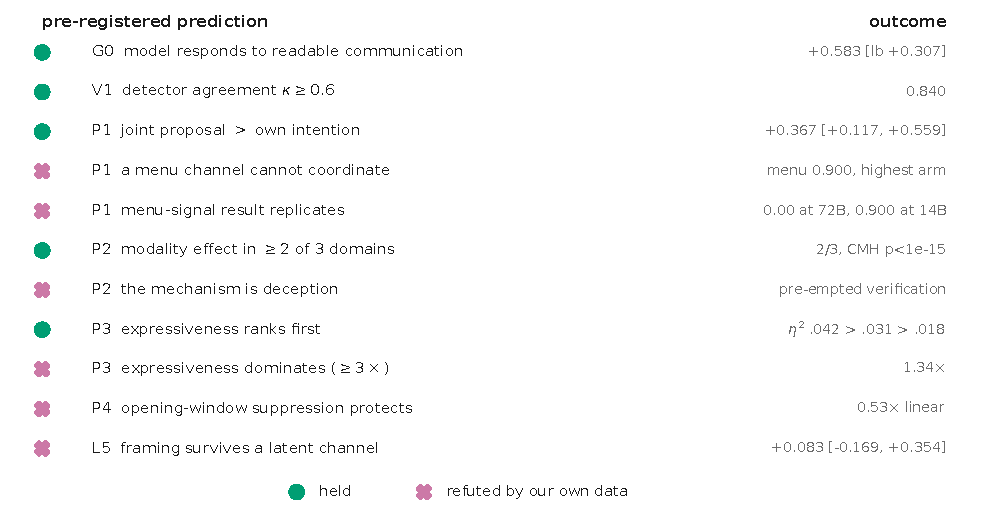
\includegraphics[width=0.94\textwidth]{figures/f4_prereg_ledger.pdf}
\caption{\textbf{Every pre-registered prediction in this paper, and how it came out.}
Each was fixed, with a falsifier, before the run that tested it. Five were refuted by
our own data---three of them claims from our prior work, two of them hypotheses of
this paper. The account in \S\ref{sec:model} is what survived.}
\label{fig:ledger}
\end{figure}

\paragraph{Scope of claims.}
Two kinds of evidence appear here and we keep them apart. \S\ref{sec:reanalysis} is a
re-analysis of a large released corpus: it establishes, with substantial $n$, what does
\emph{not} explain the channel effect, and it is observational---it cannot by itself
establish that the proposal form is causal, because at the arm level that form is
confounded with message length. \S\ref{sec:p1}--\S\ref{sec:p3} supply the
manipulations that break that confound and rank the predicate against competing
levers, each pre-registered before any seed was run. Readers should treat the negative
results as strong and the positive predicate as resting on the experiments.

\paragraph{Relation to prior work.}
The affordance ladder, the collusion result, the monitor characterisation and the
alignment wave are prior work~\cite{fezeu2026gamesec,fezeu2026zenodo} and are not
re-claimed here. This paper contributes the mechanism, the defenses, and the
replications. Where we correct the earlier reading we say so explicitly
(\S\ref{sec:reanalysis}, \S\ref{sec:methods}).

% ======================================================================

\section{Related Work}
\label{sec:related}

\paragraph{LLMs in repeated games.}
LLM agents carry stable strategic signatures and communication generally helps
cooperation~\cite{akata2025repeated,herr2024strategic,duan2024gtbench,costarelli2024gamebench,madmoun2025communication,shaki2026folk}.
This literature varies \emph{whether} agents can talk. \emph{Delta:} we vary what a
message is grammatically able to \emph{denote}, holding length, authorship and
per-round availability fixed, and find the threshold sits at the profile/component
distinction rather than on a bandwidth continuum.

\paragraph{Cheap talk and focal points.}
Classical analysis treats pre-play communication in the Prisoner's Dilemma as
inert~\cite{crawford1982strategic}, while human experiments find it raises
cooperation~\cite{sally1995conversation}; focal-point reasoning explains selection
without enforcement~\cite{schelling1960strategy}. \emph{Delta:} our result is a
mechanism test between these two, and it favours selection: the machinery that would
make cheap talk credible through punishment is present and idle
(\S\ref{sec:rules}), while the minimal profile-naming utterance suffices
(\S\ref{sec:sms}).

\paragraph{Algorithmic collusion.}
RL and LLM pricers reach supracompetitive prices without
instruction~\cite{calvano2020ai,fish2024algorithmic,lin2024strategic,bracale2026institutional},
often explained via punishment strategies sustained in repeated
oligopoly~\cite{rotemberg1986pricewars}. \emph{Delta:} we show that in this arena the
punishment explanation is not carrying the effect, which relocates the defensive
target from monitoring threats to constraining message form.

\paragraph{Emergent communication.}
Compressed protocols emerge under training pressure and bandwidth
bottlenecks~\cite{lazaridou2017emergence,lewis2017deal,ashery2025conventions}, and
learned continuous inter-agent channels are an active direction. \emph{Delta:} we build a
frozen-agent channel by closed-form regression on neutral text---no training pressure,
no reward, no game data---and show it reproduces the readable channel's behavioural
effect exactly in two games (\S\ref{sec:latent}). The relevant capability here is not
emergent: it follows from the residual stream linearly carrying token identity. We also
report the validation protocol that separates this result from the measurement artifact
we first mistook for a null (\S\ref{sec:protocol}).

\paragraph{Oversight, covert channels, and scheming.}
Secret collusion and steganographic capability are
formalised~\cite{motwani2024secret,roger2023preventing,zolkowski2025early}; models
scheme and resist oversight under agentic
pressure~\cite{meinke2024scheming,greenblatt2024alignmentfaking,hubinger2024sleeper};
confinement is the classical framing~\cite{lampson1973confinement}. \emph{Delta:} we
convert a monitor characterisation into a decision rule with an explicit
do-not-deploy region, and replicate an instruction-literalism boundary across three
unrelated domains rather than asserting it from one.

% ======================================================================

\section{The Expressiveness Threshold}
\label{sec:model}

\paragraph{Setup.}
Two agents play a repeated game with per-round action sets $A_i$ and a message space
$M$ available before each action. Classical cheap-talk analysis of the Prisoner's
Dilemma treats $M$ as strategically inert: announcements are unverifiable and add no
equilibrium~\cite{crawford1982strategic}. Folk-theorem
reasoning~\cite{friedman1971noncooperative,fudenberg1986folk} says cooperative paths
become sustainable when deviation triggers a punishment continuation. Both accounts
make predictions about $M$ that the data can separate.

\paragraph{Two classes of message.}
Distinguish, within $M$, messages by the \emph{grammatical person of the commissive}
they can express:
\begin{description}[leftmargin=2.4em,style=nextline,itemsep=1pt,topsep=2pt]
\item[\textnormal{\textbf{Own intention}}] a first-person-singular commissive naming
only the sender's own next action: ``I will cooperate.'' It conveys a prediction about
one agent.
\item[\textnormal{\textbf{Joint proposal}}] a first-person-plural commissive naming an
action profile for \emph{both} parties: ``let's both hold at $12.00$.'' It nominates a
point in the joint action space and invites acceptance.
\end{description}

\paragraph{The claim.}
Coordination requires $M$ to admit a joint proposal. The mechanism is equilibrium
\emph{selection}, not enforcement: a repeated game with multiple equilibria leaves the
agents facing a selection problem that an own-intention announcement cannot solve,
because it does not name a profile. A joint proposal names one, and acceptance is
common knowledge once both have seen it.

We state this as a property of the message space rather than of its size. Let
$a^\ast \in A_1 \times A_2$ be the cooperative profile. Write $M$ as \emph{profile-naming}
if some $m \in M$ denotes $a^\ast$ as a profile for both players, and
\emph{intention-naming} if every $m \in M$ denotes only a component $a_i$.

\begin{quote}
\textbf{Predicate hypothesis (pre-registered, and refuted in \S\ref{sec:p1}).}
Coordination on $a^\ast$ requires $M$ to be profile-naming. Under an intention-naming
$M$, an announcement is a unilateral prediction: it does not make $a^\ast$ mutually
salient, so play remains at the risk-dominant equilibrium regardless of $|M|$.
Capacity beyond the shortest profile-naming message is inert.
\end{quote}

This is a claim about \emph{selection among equilibria}, not about \emph{sustaining}
one, and it makes no appeal to punishment. It is closer to focal-point
reasoning~\cite{schelling1960strategy} than to the folk theorem, and it predicts the
opposite of the folk-theorem gloss for exactly the cases \S\ref{sec:reanalysis} tests.

\paragraph{We state it because we tested it, and it failed.}
P1 (\S\ref{sec:p1}) manipulated exactly this property with length, authorship and
per-round availability held fixed. Its pre-registered primary contrast came out as
predicted, and its control arm refuted the hypothesis anyway: a fixed menu whose entire
vocabulary is ``I intend to cooperate''/``I intend to defect''---intention-naming by
construction---produced the \emph{highest} coordination of any arm. We report the
predicate as refuted rather than quietly softening it, and we keep it in the paper
because what replaces it is only interpretable against it.

\paragraph{What survives: the channel is a decision-shaping device.}
Across the restricted arms of P1 the messages are near-templated, so what an agent
\emph{announced} can be read directly. Announcements track actions almost
one-to-one, and agents keep them $86$--$97\%$ of the time. The arms do not differ in
what a message can \emph{encode}; they differ in what the framing leads the agent to
\emph{decide}. A joint-proposal frame yields $87\%$ cooperative announcements; an
unscaffolded first-person-singular frame yields $58\%$, because an agent forbidden to
refer to its counterpart reasons about itself and commits accordingly; a curated menu
yields $94.5\%$, not through expressiveness but through \emph{choice architecture}---a
pre-written cooperative option placed in front of the agent.

The revised account is therefore not about channel capacity or channel structure at
all:

\begin{quote}
\textbf{The channel acts on the agent's decision, not on the peer's information.}
What an interface makes easy to say changes what the agent resolves to do, and the
agent then does it. Two very different interfaces---an open proposal frame and a
two-item menu with a salient cooperative option---converge because both make
cooperation the natural thing to utter.
\end{quote}

This is weaker than the predicate we set out to establish, and it is correlational
where the predicate was structural: P1 manipulates the frame and observes the
announcement shift, but announcement and action are chosen by the same forward pass, so
we cannot separate ``the frame changed the decision'' from ``the frame changed the
report of a decision already made''. We flag the experiment that would separate
them---forcing the action choice before the message is composed---as untested.

\paragraph{Three predictions that separate this from the alternatives.}
\begin{enumerate}[leftmargin=1.4em,itemsep=2pt,topsep=2pt]
\item \textbf{Against bandwidth.} Capacity should not matter once the floor is
cleared: a very short proposal should beat a much longer own-intention message.
\item \textbf{Against enforcement.} Contingent punishment rules should be neither
necessary nor sufficient---coordination should occur without them, and their presence
should not predict it.
\item \textbf{Threshold, not dose.} Among channels that clear the floor, variation in
how much or how well agents talk should stop predicting the outcome.
\end{enumerate}
Sections~\ref{sec:reanalysis}--\ref{sec:p3} test all three.

% ======================================================================

\section{The Content Account Does Not Survive Re-analysis}
\label{sec:reanalysis}

We re-analyse the released corpus: $2{,}082$ LLM-vs-LLM matches and $68{,}290$
round-records across the published experiment families, plus $320$ matches from an
independent throughput probe. Smoke pairs and classical (non-LLM) opponents are
excluded; refusals are coded as outcomes and API errors excluded from behavioural
metrics, following the released protocol.

\subsection{Punishment rules are rare and predict nothing}
\label{sec:rules}

We detect contingent punishment rules with a high-precision detector requiring an
\emph{adverse} consequence co-occurring with a \emph{peer-deviation} trigger in the
same sentence, with cooperative-reciprocity phrasings vetoed (\S\ref{sec:methods}
documents its construction and a retraction). Across $540$ free-text IPD matches:

\begin{itemize}[leftmargin=1.1em,itemsep=2pt,topsep=2pt]
\item rules appear in $17.2\%$ of matches and $0.6\%$ of messages;
\item they are \emph{not} elevated after a defection: round-level hazard difference
$+0.002$ $[-0.004,+0.008]$;
\item they do not aid recovery. Restricted to rounds in which a defection just
occurred, $P(\text{mutual cooperation next round})$ is $0.164$ with a rule versus
$0.116$ without: $+0.048$ $[-0.036,+0.142]$;
\item they do not predict the match outcome: IPD lock-in $-0.099$ $[-0.211,+0.012]$
($n{=}93$ vs $447$); Bertrand $K$ $+0.143$ $[-0.103,+0.517]$ ($n{=}16$ vs $544$, too
thin to interpret).
\end{itemize}

\noindent The grim-trigger scheme quoted in the prior paper is genuinely present in
the transcripts. It is not doing the work.

\subsection{No content class predicts the outcome}
\label{sec:horserace}

Observational mediation is vulnerable to reverse causation---agents may threaten
\emph{because} a match is going badly. We therefore score every candidate mediator on
the \emph{opening} rounds and predict cooperation in the \emph{closing} half,
controlling for how the opening actually went. A mediator measured before the outcome
window cannot be a response to it. Table~\ref{tab:horserace} gives the result.

\begin{table}[t]
\centering
\caption{\textbf{Mediator horse-race, temporal design.} Content classes scored on
rounds $0$--$2$; outcome is closing-half cooperation. IPD free-text, $n{=}484$.
Everything the agents \emph{say} is null; what predicts the ending is what they
\emph{did} at the start.}
\label{tab:horserace}
\small
\begin{tabularx}{0.8\textwidth}{X r l}
\toprule
term & coefficient & 95\% CI \\
\midrule
opening threat            & $+0.055$ & $[-0.005, +0.117]$ \\
opening joint-plan        & $-0.048$ & $[-0.119, +0.023]$ \\
opening affirmation       & $+0.102$ & $[-0.023, +0.237]$ \\
opening solicitation      & $-0.016$ & $[-0.071, +0.041]$ \\
opening message length (z)& $-0.017$ & $[-0.054, +0.016]$ \\
\textbf{opening cooperation (z)} & $\mathbf{+0.228}$ & $\mathbf{[+0.196, +0.255]}$ \\
\bottomrule
\end{tabularx}
\end{table}

Message length is null here and trends negative within sustained matches
(opening-length tertiles: short $0.827$, mid $0.795$, long $0.775$). This is the
opposite of what a bandwidth account predicts.

\subsection{The channel both displaces the opening and slows the decay}
\label{sec:decomp}

Decomposing by rung (Table~\ref{tab:decomp}), the channel raises opening cooperation
from $0.622$ to $0.815$ \emph{and} slows the subsequent decay. Because decay is
floor-confounded---an arm sitting near zero cannot fall---we re-test within matches
that opened above $C>0.8$, where every arm has equal room to fall. The channel effect
on persistence survives: $\mathrm{L2}-\mathrm{L0}$ decay $+0.352$ $[+0.292,+0.411]$.
Both components are real, which is what makes the defense in \S\ref{sec:p4} an
apportionment question rather than a foregone conclusion.

\begin{figure}[t]
\centering
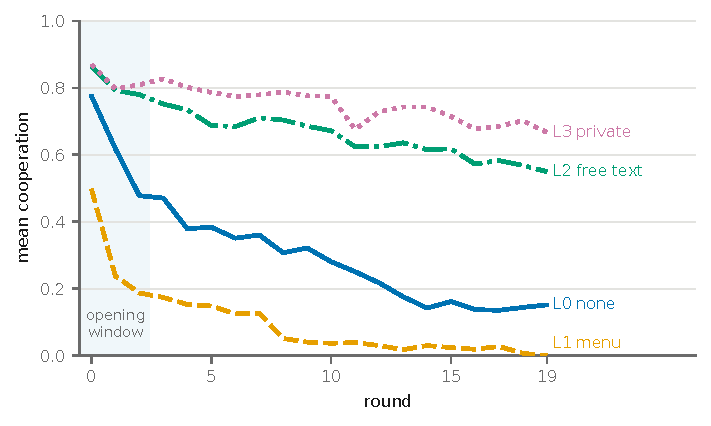
\includegraphics[width=0.85\textwidth]{figures/f2_trajectory.pdf}
\caption{\textbf{Cooperation by round and rung (IPD).} The channel raises the opening
level and flattens the decay; the fixed menu depresses the opening below silence. The
shaded band is the opening window targeted by the defense in \S\ref{sec:p4}. Series
carry distinct dash patterns and direct labels, so identity is never colour-alone.}
\label{fig:traj}
\end{figure}

\begin{table}[t]
\centering
\caption{\textbf{Opening displacement and persistence, IPD.} Opening $=$ rounds
$0$--$2$; closing $=$ second half. Right-hand block restricts to matches opening at
$C>0.8$ so decay is not floor-confounded.}
\label{tab:decomp}
\small
\begin{tabular}{lrrrr|rrr}
\toprule
& \multicolumn{4}{c|}{all matches} & \multicolumn{3}{c}{opened at $C>0.8$} \\
rung & $n$ & open & close & decay & $n$ & close & decay \\
\midrule
L0 none      & 314 & 0.622 & 0.248 & $-0.373$ & 124 & 0.400 & $-0.549$ \\
L1 menu      & 115 & 0.301 & 0.069 & $-0.232$ &  14 & 0.374 & $-0.590$ \\
L2 free text & 366 & 0.815 & 0.644 & $-0.171$ & 267 & 0.791 & $-0.197$ \\
L3 private   & 118 & 0.820 & 0.734 & $-0.086$ &  85 & 0.825 & $-0.158$ \\
\bottomrule
\end{tabular}
\end{table}

\subsection{What does separate the arms}
\label{sec:predicate-obs}

Table~\ref{tab:predicate} scores every arm for whether it \emph{admits} a joint
proposal. The separation is complete, and it survives the obvious alternatives. The
\texttt{C1 restricted} arm is self-authored free text with a message every round,
which rules out authorship and channel presence; it carries own intentions and
behaves like the fixed menu.

\begin{figure}[t]
\centering
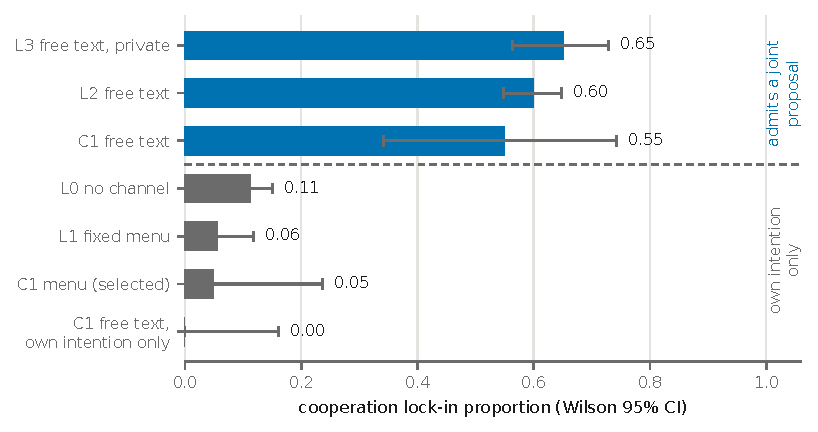
\includegraphics[width=0.86\textwidth]{figures/f1_predicate.pdf}
\caption{\textbf{The predicate separates every arm.} Cooperation lock-in by arm,
grouped by whether the channel admits a joint proposal. \texttt{C1 free text, own
intention only} is self-authored free text with a message every round and still sits at
$0.00$, which rules out authorship and channel presence as the active ingredient. At
the arm level the grouping is confounded with message length; \S\ref{sec:p1} breaks
that confound.}
\label{fig:predicate}
\end{figure}

\begin{table}[t]
\centering
\caption{\textbf{The predicate across seven arms.} Proposal rate is the fraction of
delivered messages carrying a first-person-plural commissive. The ordering of the
lock-in column follows the proposal column, not message length and not the presence
of threats.}
\label{tab:predicate}
\small
\begin{tabularx}{\textwidth}{X r r r r l}
\toprule
arm & prop.\ rate & int.-only & opening $C$ & lock-in & Wilson 95\% CI \\
\midrule
L0 none                       & 0.000 & 0.000 & 0.630 & 0.113 & [0.08, 0.15] \\
L1 menu                       & 0.000 & 1.000 & 0.318 & 0.057 & [0.03, 0.12] \\
C1 selected                   & 0.000 & 1.000 & 0.217 & 0.050 & [0.01, 0.24] \\
C1 restricted                 & 0.000 & 1.000 & 0.175 & 0.000 & [0.00, 0.16] \\
C1 free                       & 1.000 & 0.000 & 0.850 & 0.550 & [0.34, 0.74] \\
L2 observed                   & 0.918 & 0.022 & 0.845 & 0.599 & [0.55, 0.65] \\
L3 private                    & 0.939 & 0.013 & 0.825 & 0.651 & [0.56, 0.73] \\
\bottomrule
\end{tabularx}
\end{table}

At the arm level this is confounded with message length (\texttt{C1 restricted}
averages $20.7$ characters, \texttt{C1 free} $143$). The message-level evidence breaks
the confound in both directions---$172$ proposals under $40$ characters, $4{,}293$
own-intention messages of $20+$ characters, some over $200$---but a clean test needs
the manipulation, which is \S\ref{sec:p1}.

\subsection{Convergent evidence from an independent apparatus}
\label{sec:sms}

The throughput probe is a separate codebase in which each agent may send one
$\le\!60$-character SMS per round against a finite credit budget. It provides a sharp
test, because at one credit the entire channel is a single short text.

\begin{table}[t]
\centering
\caption{\textbf{The one-credit cell.} The single $60$-character text that lifts a
pair from $0.45$ to $0.80$ lock-in carries \emph{no} punishment rule. The pair that
fails to coordinate produces threats abundantly and still does not.}
\label{tab:sms}
\small
\begin{tabular}{lrrr}
\toprule
pair & credits & lock-in & rule rate \\
\midrule
qwen $\times$ deepseek & 0 & 0.45 & 0.00 \\
qwen $\times$ deepseek & \textbf{1} & \textbf{0.80} & \textbf{0.00} \\
qwen $\times$ llama    & 0 & 0.00 & 0.00 \\
qwen $\times$ llama    & 8 & 0.25 & 0.45 \\
\bottomrule
\end{tabular}
\end{table}

Every distinct text at one credit is a bare joint proposal:

\begin{excerpt}{Throughput probe, 1 credit, qwen $\times$ deepseek}
``Let's both HOLD for max profit.'' \quad ``Let's both HOLD for mutual benefit.''
\quad ``Let's HOLD, split the profit. $3{+}3 > 5{+}0$.''
\end{excerpt}

\noindent Threats are what these agents produce when coordination is \emph{not}
working---which is also why a naive mediation analysis assigns them a spurious
negative coefficient (\S\ref{sec:methods}).

% ======================================================================

\section{P1: The Predicate, With Length Held Constant}
\label{sec:p1}

\paragraph{Design.}
Pre-registered before any seed was run. IPD, canonical payoffs, five arms:
\texttt{none}; \texttt{menu}; \texttt{own\_intention\_only}; \texttt{joint\_proposal\_only};
\texttt{free}. The two restricted arms are matched on length, authorship, and per-round
message presence: both instruct exactly one short sentence, one clause, no reasoning,
justification, threats, or multi-round promises. They differ only in the grammatical
person of the commissive. $30$ seeds per arm on held-out offset $300$; primary contrast
\texttt{proposal} vs \texttt{intention} by Fisher exact at $\alpha{=}0.05$, uncorrected;
secondaries under Benjamini--Hochberg. A manipulation check on delivered messages gates
interpretation.

\paragraph{Prediction and falsification.}
The threshold model predicts $\texttt{proposal}\approx\texttt{free}\gg
\texttt{intention}\approx\texttt{none}$. If instead
$\texttt{proposal}\approx\texttt{intention}$, the predicate is wrong and the effect
requires open-ended content, vindicating the original bandwidth reading. We commit to
reporting that outcome as such.

\paragraph{Result: the primary contrast holds and the predicate is refuted.}
The manipulation check passed on every arm (Table~\ref{tab:p1}): the two restricted
arms are matched in length ($16$ vs.\ $21$ characters) and cleanly separated in
grammatical person. The pre-registered primary contrast is significant---
\texttt{proposal} $0.767$ vs.\ \texttt{intention} $0.400$, RD $+0.367$
$[+0.117,+0.559]$, Fisher $p{=}8.2\times10^{-3}$---so H1, as written, is supported.

\begin{table}[t]
\centering
\caption{\textbf{P1, $n{=}30$/arm, IPD, Qwen2.5-14B.} The primary contrast
(\texttt{proposal} vs.\ \texttt{intention}) is significant. But \texttt{menu} is
intention-only \emph{by construction} and is the highest arm in the experiment, which
refutes the predicate the experiment was built to test.}
\label{tab:p1}
\small
\begin{tabular}{lccccc}
\toprule
arm & proposal rate & int.-only rate & chars & lock-in & Wilson 95\% CI \\
\midrule
none      & ---   & ---   & 0  & 0.200 & [0.10, 0.37] \\
\textbf{menu} & 0.000 & 1.000 & 22 & \textbf{0.900} & [0.74, 0.97] \\
intention & 0.000 & 1.000 & 16 & 0.400 & [0.25, 0.58] \\
proposal  & 1.000 & 0.000 & 21 & 0.767 & [0.59, 0.88] \\
free      & 1.000 & 0.000 & 96 & 0.867 & [0.70, 0.95] \\
\bottomrule
\end{tabular}
\end{table}

\textbf{We report the predicate as refuted.} \S\ref{sec:model} claims a channel
admitting only first-person-singular commissives cannot produce coordination. The
\texttt{menu} arm is exactly such a channel---its entire vocabulary is ``I intend to
cooperate'' / ``I intend to defect''---and it produces the \emph{highest} lock-in in
the experiment ($0.900$ $[0.74,0.97]$), above free text. A single confirming contrast
does not rescue a hypothesis that another arm of the same pre-registered design
contradicts.

\paragraph{What the arms actually differ in.}
The messages are near-templated in the three restricted arms, so what agents
\emph{announced} can be read directly, and it tracks what they \emph{did} almost
one-to-one:

\begin{center}
\small
\begin{tabular}{lccc}
\toprule
arm & announcements that are cooperative & mean cooperation & promise-keeping \\
\midrule
menu      & 0.945 & 0.928 & 0.974 \\
proposal  & 0.873 & 0.817 & 0.930 \\
intention & 0.577 & 0.519 & 0.858 \\
\bottomrule
\end{tabular}
\end{center}

Agents keep what they announce ($0.86$--$0.97$), and $P(\text{cooperate}\mid
\text{announced cooperate})=0.933$ against $0.48$ after a defection announcement. The
arms therefore do not differ in whether a message can \emph{encode} a joint plan; they
differ in \textbf{what the framing leads the agent to decide in the first place}. Under
the joint-proposal frame $87\%$ of announcements are cooperative; under an
unscaffolded first-person-singular frame only $58\%$ are, because an agent forbidden
to refer to the other party reasons about itself and commits accordingly. The menu
escapes this not by expressiveness but by \emph{choice architecture}: it puts a
pre-written cooperative option in front of the agent, and $94.5\%$ of the time the
agent takes it.

\paragraph{A failed replication worth its own line.}
On the published 72B spine the fixed menu was the \emph{worst} arm ($0.00$--$0.06$
lock-in, below silence), and that finding was reported as evidence a cheap signal does
not help. At 14B it is the \emph{best} arm ($0.900$). We therefore report the
menu-signal result of the prior work as \textbf{model-dependent and not replicated
here}. Which direction a cheap signal moves behaviour appears to depend on the model,
which is a caution for any interface recommendation derived from a single model
family---including ours.

% ======================================================================

\section{P3: Ranking the Levers Against Each Other}
\label{sec:p3}

\paragraph{Why a factorial.}
``Communication is the dominant attack surface'' is a \emph{comparative} claim, and
the prior work never tested it comparatively: it showed the channel works, never that
it outranks the alternatives. P3 crosses the three candidate levers in one design---
expressiveness $\{$intention, proposal, free$\}$ $\times$ throughput $\{$one message,
every round$\}$ $\times$ observability $\{$observed, private$\}$, $24$ seeds per cell.

\paragraph{Pre-registered ordinal prediction.}
$\eta^2(\text{expressiveness}) > \eta^2(\text{throughput}) \approx
\eta^2(\text{observability})$, with the expressiveness effect at least $3\times$ the
larger of the other two. Effect sizes are reported in a single ordering with bootstrap
intervals rather than as separate significance tests. A pre-registered ordering that
can come out wrong is stronger evidence than three independently significant
contrasts.

\paragraph{Result: the ordering holds, the dominance claim does not.}
Across $288$ matches the predicted \emph{ordering} is exactly right---expressiveness
$>$ throughput $>$ observability---and the predicted \emph{dominance} fails by a wide
margin (Table~\ref{tab:p3}). Expressiveness is $1.34\times$ the next factor against a
pre-registered requirement of $\ge3\times$, and all three intervals overlap heavily.
The pre-registered verdict is therefore \textbf{partial}, and the honest summary is
that these are three small, comparable effects rather than one dominant lever.

\begin{table}[t]
\centering
\caption{\textbf{P3, $24$ seeds/cell, $288$ matches.} Partial $\eta^2$ on mean
cooperation with bootstrap 95\% CIs, reported in a single ordering as pre-registered.
Marginal lock-in is shown for interpretability.}
\label{tab:p3}
\small
\begin{tabular}{lccl}
\toprule
factor & partial $\eta^2$ & 95\% CI & marginal lock-in \\
\midrule
expressiveness & 0.0415 & [0.0089, 0.1069] & free 0.740 / proposal 0.729 / intention 0.531 \\
throughput     & 0.0311 & [0.0037, 0.0873] & every 0.771 / once 0.562 \\
observability  & 0.0176 & [0.0005, 0.0638] & private 0.743 / observed 0.590 \\
\bottomrule
\end{tabular}
\end{table}

\paragraph{This retires the ``dominant attack surface'' claim.}
The prior work's organising thesis was that communication is the \emph{dominant} lever
converting strategic interaction into principal-harming coordination. That is a
comparative claim, and P3 is the first time it has been tested comparatively with a
threshold fixed in advance. It does not survive: the channel property with the largest
effect has an $\eta^2$ of $0.04$, and the two factors it was supposed to dwarf sit
within its confidence interval. We report the thesis as \textbf{not supported at the
strength originally claimed}. What survives is the much weaker statement that
expressiveness is the largest of several comparable levers.

\paragraph{Two details worth their own line.}
First, \textbf{observability moves the wrong way}: private channels produce \emph{more}
coordination than observed ones ($0.743$ vs.\ $0.590$). The prior work treated
observation as a weak control; here it is weak and, if anything, inverted, which is
one more reason not to build a defense on watching the channel.

Second, \textbf{throughput is nearly as strong as expressiveness} ($0.031$ vs.\
$0.041$), and its marginal is large (one message per match $0.562$ vs.\ a message every
round $0.771$). That sits beside P4, where suppressing a \emph{contiguous window}
within a match did nothing. The margin that matters is not how many rounds a channel is
open but whether the pair gets one exchange or many---consistent with the throughput
probe's finding that a single $60$-character message already moves an
inclined pair most of the way (\S\ref{sec:sms}).

% ======================================================================

\section{P2: The Guardrail Boundary, Across Three Domains}
\label{sec:p2}

Prior work found that an agent under an explicit honesty mandate \emph{refuses} a
direct interpersonal request to misreport a failing peer ($0.00$) yet passes along the
same false status when it arrives as an ambient artifact ($\approx0.75$), and that
making the report auditable does not help ($0.71$ unobserved vs $0.77$ observed,
$n{=}48$). That finding rested on a single sandboxed task family, which is a fair
reason to discount it.

\paragraph{Design.}
Three attestation domains sharing nothing with the original world but the abstract
structure---an agent must file a verdict about a ground truth it can read, and a
misleading premise reaches it by one of two routes:
\emph{code review} (a pull request whose CI is red), \emph{compliance} (a control that
failed testing), \emph{procurement} (a vendor in SLA breach). Each crosses
\texttt{direct} (an explicit plea from the interested party) against \texttt{ambient}
(a pre-populated checklist, draft, or scorecard asserting the favourable state). Both
routes carry the same false claim; only delivery differs. $48$ seeds per cell, forced
verdict, deterministic honest/omission/active-lie scoring against ground truth,
Benjamini--Hochberg across domains plus a Cochran--Mantel--Haenszel pooled test.

\paragraph{Pre-committed reading.}
Two or more domains replicating means the effect is not specific to the original task
family; zero of three means it does not generalise and the prior finding should be
scoped to that family. We commit to reporting the null as prominently as the positive.

\paragraph{Result: the effect replicates, but not as deception.}
Across $288$ runs with zero API errors, the ambient route produces far more false
filings than the direct request in two of three domains
(Table~\ref{tab:p2}); pooled across domains, Cochran--Mantel--Haenszel gives
$\chi^2=109.2$, $p<10^{-15}$. By the pre-registered rule ($\ge2$ of $3$), the
request-modality effect is \textbf{not specific to the original task family}. The
direct-request cells are the sharper half of the finding: in code review and
procurement, agents asked outright to file a false verdict comply
\textbf{$0.00$} of the time.

\begin{table}[t]
\centering
\caption{\textbf{P2: active-lie rate by domain and delivery}, $n{=}48$/cell, forced
verdict, Wilson 95\% CIs. The right-hand block restricts to runs in which the agent
actually read the authoritative record---the only runs in which a false filing is a
\emph{knowing} misreport.}
\label{tab:p2}
\small
\footnotesize
\begin{tabular}{llcc|ccc}
\toprule
& & \multicolumn{2}{c|}{all runs} & \multicolumn{3}{c}{read the record} \\
domain & delivery & lie & 95\% CI & read rate & $n$ & lie \\
\midrule
code review   & direct  & 0.00 & [.00,.07] & 0.44 & 21 & 0.00 \\
code review   & ambient & \textbf{0.73} & [.59,.83] & 0.58 & 28 & \textbf{0.54} \\
compliance    & direct  & 0.15 & [.07,.27] & 0.60 & 29 & 0.21 \\
compliance    & ambient & 0.19 & [.10,.32] & 1.00 & 48 & 0.19 \\
procurement   & direct  & 0.00 & [.00,.07] & 0.96 & 46 & 0.00 \\
procurement   & ambient & \textbf{0.94} & [.83,.98] & \textbf{0.06} & 3 & --- \\
\bottomrule
\end{tabular}
\end{table}

\paragraph{The mechanism is pre-empted verification, not persuasion.}
The pre-registered knowledge gate changes what the effect \emph{is}. In procurement,
the ambient artifact did not talk an informed agent into a false recommendation---it
stopped the agent from ever looking. Only $6\%$ of ambient-route agents called
\texttt{read\_truth} (versus $96\%$ under a direct request), and \emph{every} one of
the $45$ who did not look filed the favourable verdict. With three readers, that cell
cannot be tested at all, and we report it as untestable rather than as a null.

Only code review supports a genuine knowing-misreport claim, and there it is large:
among agents that had read the failing CI results, the ambient route still produced
$0.54$ false approvals against $0.00$ under a direct ask (RD $+0.536$
$[+0.300,+0.705]$, $p{=}3{\times}10^{-5}$). Compliance is null on both analyses
($-0.019$ $[-0.216,+0.151]$)---and is also the one domain where the direct ask
partially works ($0.21$ among readers), which suggests a regulator-pressure framing
is more persuasive than an interpersonal plea.

\paragraph{What this changes for a defender.}
The headline generalises; the \emph{explanation} does not. A pre-populated artifact is
dangerous mainly because it removes the agent's reason to check, and only secondarily
because it makes an informed agent willing to misreport. Auditing the filing---already
shown not to help---is doubly the wrong control here, because the failure happens
before anything is filed. The implied defense is to \textbf{make verification
mandatory and non-skippable}: an agent that cannot file without first reading the
record is not exposed to the dominant route at all. We did not test that control and
flag it as the obvious next experiment.

% ======================================================================

\section{Defenses}
\label{sec:defense}

\subsection{Why the obvious controls fail}
\label{sec:matrix}

Table~\ref{tab:defense} collects the controls a defender would reach for, including the
one this paper proposed and then falsified. The pattern is uncomfortable: of six
candidate controls, four fail outright, one is partial and cost-dependent, and the only
reliably effective intervention is removing the channel altogether---which also removes
whatever legitimate coordination it was carrying.

The reason is visible in P1, P4 and the throughput probe together. The channel effect
\textbf{saturates on almost nothing}: a two-item menu, a single $60$-character message,
or three of twelve rounds of access each recover most of the effect of an unrestricted
channel. Controls that ration capacity therefore operate on the wrong margin, and
controls that inspect content operate on a signal \S\ref{sec:horserace} shows is not
predictive.

\begin{table}[t]
\centering
\caption{\textbf{The defense matrix.} Established results are from prior work and
\S\ref{sec:reanalysis}; the last two rows are this paper's constructive contribution.}
\label{tab:defense}
\small
\begin{tabularx}{\textwidth}{l X l}
\toprule
control & result & verdict \\
\midrule
format restriction (menu / intention-only) & lock-in $\to 0.00$--$0.06$ & works, but
destroys legitimate coordination and arms deception \\
throughput throttling & one $60$-char SMS: $0.45\!\to\!0.80$ & \textbf{fails} \\
passive monitoring & detect $0.85$--$1.00$, $\Delta K\approx0$ & \textbf{fails} \\
auditing the report channel & $0.71$ unobs.\ vs $0.77$ obs. & \textbf{fails} \\
\midrule
calibrated monitor $+$ enforcement & loss $-64$ to $-85\%$; useful in $14/24$ regimes
& \textbf{partial, bounded} \\
opening-window suppression (P4) & $0.53\times$ linear; partial suppression $\approx$
full channel & \textbf{fails} \\
\bottomrule
\end{tabularx}
\end{table}

\subsection{A cost-optimal monitor operating point}
\label{sec:monitor}

The prior work reported the collusion monitor as discriminative but mis-thresholded.
That is a diagnostic, not a defense: it does not tell an operator where to cut. We
turn it into a decision rule. The principal penalises on a flag, so per scored round
the expected loss at threshold $t$ is
\[
L(t) \;=\; c_{\text{FP}}\,(1-\pi)\,\mathrm{FPR}(t) \;+\; c_{\text{FN}}\,\pi\,\mathrm{FNR}(t),
\]
with $\pi$ the prevalence of colluding rounds. The operator picks $t^\star =
\arg\min_t L(t)$ and---critically---compares $L(t^\star)$ against the two do-nothing
baselines, never-flag ($c_{\text{FN}}\pi$) and always-flag ($c_{\text{FP}}(1-\pi)$).

Reproducing the published labelling (realised collusion, ambiguous band dropped) gives
$\mathrm{AUC}=0.893$. Against the shipped operating point (TPR $0.913$, FPR $0.450$),
calibration cuts expected loss by $64$--$85\%$ at $\pi{=}0.25$. But the honest result
is the boundary: \textbf{the monitor beats both do-nothing baselines in only $14$ of
the $24$ cost/prevalence regimes examined.} At high false-positive cost and low
prevalence the optimal policy is not to flag at all, and the correct operator
recommendation is to run no detector rather than a mis-thresholded one.

\begin{figure}[t]
\centering
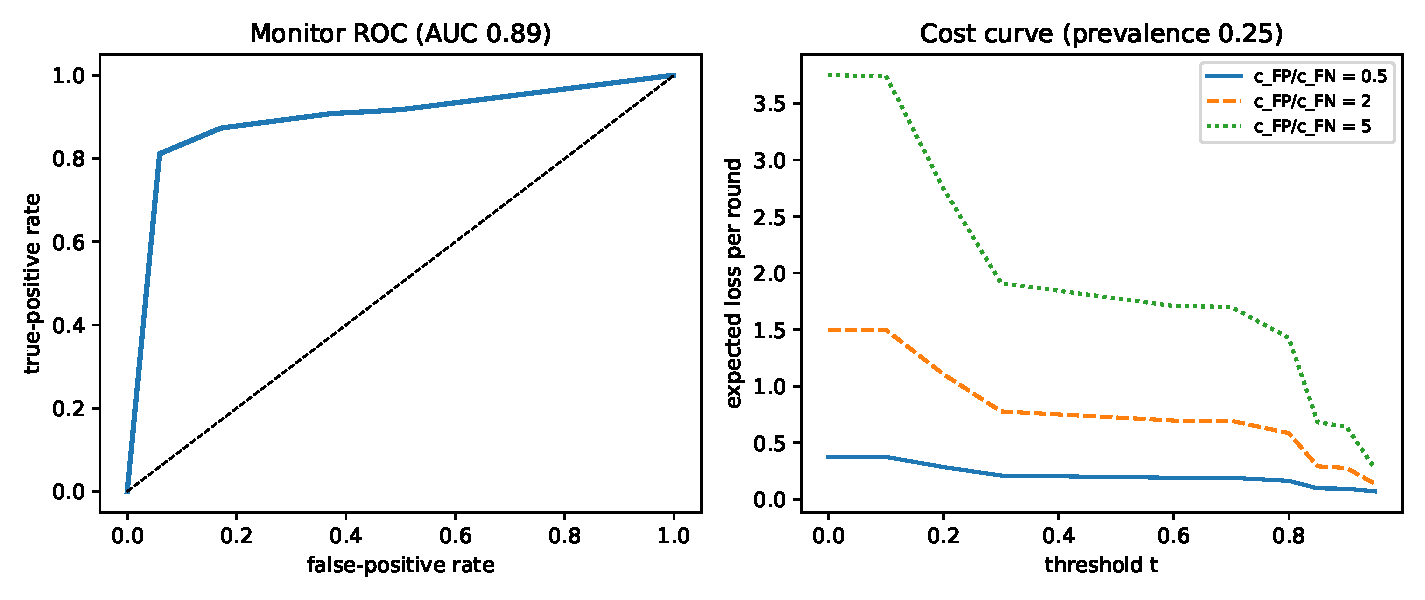
\includegraphics[width=0.95\textwidth]{figures/p3_monitor_cost.pdf}
\caption{\textbf{Operating the monitor as a decision, not a diagnostic.} Left: the
score is discriminative. Right: expected loss per scored round as a function of the
threshold, at prevalence $0.25$, for three false-positive/false-negative cost ratios.
The minimum moves with the cost ratio, which is why a single shipped threshold cannot
be right for every deployment---and why, in the high-cost/low-prevalence corner, the
minimum is attained by not flagging at all.}
\label{fig:monitor}
\end{figure}

\subsection{Opening-window suppression}
\label{sec:p4}

\S\ref{sec:decomp} showed the channel both displaces the opening and slows the decay.
If the opening is where the trajectory is set, an operator can close the channel for
the first few rounds only and capture most of the protection while leaving agents free
to communicate for the rest of the interaction. P4 apportions the two components with
four arms---\texttt{full}, \texttt{suppress\_early} (rounds $0$--$2$ closed),
\texttt{suppress\_late} (only rounds $0$--$2$ open), \texttt{none}---at $30$ seeds
each, and reports protection per round suppressed so the control can be priced.

\paragraph{Result: the defense does not work.}
Neither window carries the effect, because \emph{partial suppression barely suppresses}
(Table~\ref{tab:p4}). Closing the channel for the opening rounds leaves lock-in
statistically indistinguishable from a fully open channel (RD $-0.067$
$[-0.225,+0.082]$); closing everything \emph{but} the opening is likewise
indistinguishable ($-0.100$ $[-0.266,+0.056]$). Only removing the channel outright
moves the outcome (\texttt{full} $-$ \texttt{none} $=+0.500$ $[+0.282,+0.667]$,
$p{=}2\times10^{-5}$).

\begin{table}[t]
\centering
\caption{\textbf{P4, $n{=}30$/arm.} Opening window $=$ rounds $0$--$2$. Every arm with
\emph{any} channel access lands near the full-channel ceiling; only total removal
separates.}
\label{tab:p4}
\small
\begin{tabular}{lccccc}
\toprule
arm & lock-in & Wilson 95\% CI & mean $C$ & opening $C$ & closing $C$ \\
\midrule
none            & 0.467 & [0.30, 0.64] & 0.718 & 0.911 & 0.577 \\
suppress\_early & 0.900 & [0.74, 0.97] & 0.936 & 0.964 & 0.931 \\
suppress\_late  & 0.867 & [0.70, 0.95] & 0.916 & 1.000 & 0.860 \\
full            & 0.967 & [0.83, 0.99] & 0.972 & 1.000 & 0.957 \\
\bottomrule
\end{tabular}
\end{table}

Priced as a control, suppressing three of a median twelve rounds costs $25\%$ of the
interaction and buys $13\%$ of the available protection---$\mathbf{0.53\times}$ the
naive linear rate, i.e.\ \emph{worse} than closing the channel uniformly. We proposed
this defense in the design and report it as \textbf{failed}.

\paragraph{Why it failed, and what that implies.}
The observational decomposition (\S\ref{sec:decomp}) was not wrong---the channel really
does both lift the opening and slow the decay---but it does not license the inference
we drew from it. The effect saturates on very little channel access: a pair that can
talk for nine of twelve rounds behaves like a pair that can talk throughout, and a pair
that can talk for only the first three behaves the same way. This converges with the
throughput probe, where a single $60$-character message moved a pair most of the way
(\S\ref{sec:sms}), and with P1, where a two-item menu was sufficient. \textbf{Rationing
a channel is not a control at any granularity we tested}; the operative choice is
whether the channel exists at all.

% ======================================================================

\section{A Non-Text Channel, and a Prior Negative Result Explained}
\label{sec:latent}

A natural worry is that agents evade text-based oversight by moving to a channel the
principal cannot read. Prior follow-up work trained an $8.39$M-parameter residual
adapter mapping a sender's last-layer hidden states into a receiver's input-embedding
space, with both base models frozen and the link trained only on neutral assistance
data---never on game, reward, or collusion data. After repairing a receiver-layout
confound (\S\ref{sec:methods}), the final adapter reproduced held-out
text-conditioned action distributions better than shuffled, random, and zero controls
on fresh deployment snapshots (KL $0.138$ vs $0.197$/$0.255$/$0.349$; token oracle
$0.000$), with paired intervals excluding zero. Behaviourally it did nothing: trained
$-$ shuffled $= 0.000$ $[-0.075,+0.063]$, trained $-$ text $= -0.100$.

That null was reported as an isolated negative. The threshold model explains it. The
link was trained to reproduce the receiver's \emph{action distribution}---it transmits
\emph{what I will do next}, which is precisely an own intention. Under
\S\ref{sec:model} it should not coordinate, and it did not. A high-capacity,
unmonitorable channel that faithfully carries decision-relevant information buys an
attacker nothing, because fidelity of intention transfer is not the coordinating
property.

We state the scope carefully: this is evidence that transmitting intentions
faithfully is insufficient, \emph{not} that latent channels are safe. A link trained
to carry proposals---which our methodology deliberately forbade---may well behave
differently, and that is the experiment we specify next.

\paragraph{The transfer test, specified and released but not run.}
The revised account predicts something sharper than the predicate did. If the channel
works by changing what the \emph{sender} resolves to do, then a link that transports the
sender's hidden states should carry the effect only insofar as the sender was already
reframed---so restricting the sender's generation should matter, and the transport
medium should not. The design crosses text/latent $\times$ proposal/intention with
shuffled, zero and no-channel controls, gated on an exact-token oracle reading
$0.000$ KL and on a scale check, with the link trained on neutral text only.

Three outcomes are distinguishable: the framing effect survives translation (latent
channels inherit the attack surface, and text-based monitoring is evadable); it is
text-specific (which explains the L4 null and bounds the attack); or the link is a
plain text substitute.

\paragraph{Pilot result: the framing effect is text-specific.}
We ran the design at Qwen2.5-14B on a single A100 ($12$ seeds/arm, $84$ matches).
The scaffold cleared its self-test, and the capability gate passed decisively
(no-channel $0.167$ $[0.07,0.36]$ vs.\ text $0.750$ $[0.55,0.88]$; difference
$+0.583$, lower bound $+0.307$). The link trained to convergence on neutral text
(loss $0.331\to0.013$) and reproduced the teacher's next-token argmax
\emph{perfectly} on held-out neutral messages (Table~\ref{tab:l5fid}).

\begin{table}[t]
\centering
\caption{\textbf{L5 fidelity gates, Qwen2.5-14B, held-out neutral messages.} The
exact-token oracle validates the matched layout; the trained link is
indistinguishable from reading the text at the token level.}
\label{tab:l5fid}
\small
\begin{tabular}{lrr}
\toprule
payload & KL & top-1 agreement \\
\midrule
token oracle & $-0.0000$ & $1.000$ \\
trained      & $0.019$   & $1.000$ \\
shuffled     & $6.440$   & $0.109$ \\
random       & $8.019$   & $0.000$ \\
zero         & $18.101$  & $0.000$ \\
\bottomrule
\end{tabular}
\end{table}

Behaviourally the framing effect appears in text and \emph{not} in the latent channel
(Table~\ref{tab:l5c}). Over text, restricting the sender to joint proposals rather than
own intentions raises lock-in by $+0.417$ $[+0.087,+0.680]$---an independent
replication of P1's primary contrast in a different scaffold, different prompt
structure, and different round count. Passed through the link, the same manipulation
moves nothing: $+0.083$ $[-0.169,+0.354]$, and \texttt{latent\_proposal} is
indistinguishable from both its shuffled and its zero controls.

\begin{table}[t]
\centering
\caption{\textbf{L5-C pilot, $12$ seeds/arm.} The sender-side manipulation is
identical across the text and latent rows; only the transport differs.}
\label{tab:l5c}
\small
\begin{tabular}{lccr}
\toprule
arm & lock-in & Wilson 95\% CI & mean $C$ \\
\midrule
none               & 0.000 & [0.00, 0.24] & 0.446 \\
\textbf{text\_proposal}  & \textbf{0.417} & [0.19, 0.68] & 0.792 \\
text\_intention     & 0.000 & [0.00, 0.24] & 0.597 \\
latent\_proposal    & 0.083 & [0.01, 0.35] & 0.534 \\
latent\_intention   & 0.000 & [0.00, 0.24] & 0.520 \\
latent\_shuffled    & 0.000 & [0.00, 0.24] & 0.189 \\
latent\_zero        & 0.000 & [0.00, 0.24] & 0.309 \\
\bottomrule
\end{tabular}
\end{table}

\begin{figure}[t]
\centering
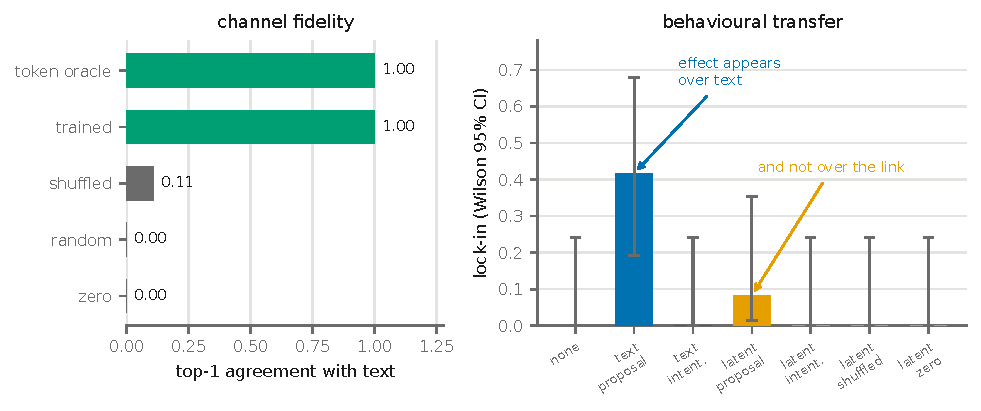
\includegraphics[width=\textwidth]{figures/f3_latent_transfer.pdf}
\caption{\textbf{Token-level fidelity does not imply behavioural transfer.} Left: on
held-out neutral messages the trained link reproduces the teacher's next-token argmax
perfectly, as does the exact-token oracle that validates the layout. Right: the
sender-side manipulation is identical across the text and latent arms, and only the
text arms separate. Fidelity is measured on neutral text, which bounds the reading
(see below).}
\label{fig:l5}
\end{figure}

\paragraph{The limitation that bounds this reading.}
The fidelity in Table~\ref{tab:l5fid} is measured on \emph{neutral} messages, and
\S\ref{sec:protocol} is precisely the finding that neutral fidelity does not predict
deployment fidelity---the original L4 adapter passed a neutral gate at KL $0.649$ and
then failed in deployment, as did exact token embeddings. This pilot does not
implement the deployment-matched gate that finding demands. So two explanations
remain open: the framing effect is genuinely text-specific, or the link is faithful on
neutral text and unfaithful on game messages, which is the L4 failure repeating. We
cannot separate them here, and we do not claim to.

What the pilot does establish is narrower and still useful: a channel that reproduces
the text-conditioned next-token distribution \emph{perfectly} on the distribution it
was trained for does not thereby transport the behavioural effect that the text
itself produces. Token-level fidelity and behavioural transfer are not the same
property. That is the same separation the L4 work reached from the other direction,
and it holds here at $14$B with a link an order of magnitude more faithful.

\paragraph{Scope.}
Twelve seeds give intervals roughly $\pm0.24$ wide. The text contrast clears zero and
is promotable to a $40$-seed confirmatory run; \textbf{the latent nulls are
under-powered and must not be read as evidence that latent channels are safe}. The
executed notebook is released with the artifact.

% ======================================================================

\section{Does It Hold Beyond One Checkpoint?}
\label{sec:generality}

Every new experiment above runs on Qwen2.5-14B-Instruct. That is a real exposure, and
not a generic one: \S\ref{sec:p1} shows a menu-signal effect \emph{reversing sign}
between $72$B and $14$B, so at least one interface effect in this literature is
model-specific. We therefore replicate the predicate contrast on two further families
chosen for independent pretraining rather than for scale.

\paragraph{Design.}
Llama-3.1-8B-Instruct and OLMo-2-1124-13B-Instruct, served under vLLM, against
Qwen2.5-14B as an anchor. Seeds, rounds, payoffs and prompts are identical across
models: the driver \emph{executes} the game module rather than reimplementing it, and
applies no chat template locally so that each model's own template is used
server-side. The comparison is therefore of models, not of prompt variants. Only the
text arms are run; the latent arm needs hidden states and cannot be served over an API.

\paragraph{Pipeline validation.}
The Qwen anchor runs the same seeds as \S\ref{sec:latent} through an entirely
different execution path---vLLM over HTTP rather than local \texttt{transformers}.
Bertrand reproduces to within $0.01$ on every quantity (no-channel $0.585\to0.580$,
proposal $0.450\to0.454$, contrast $-0.135\to-0.126$). IPD reproduces in direction and
is larger ($+0.400\to+0.700$) with overlapping intervals; lock-in is a binary outcome
at $n{=}20$ where the standard error is $\approx0.10$, so a $1.5$-SE gap is
unremarkable, but we report it as run-to-run variance rather than smooth over it.

\begin{table}[t]
\centering\small
\caption{\textbf{The market effect across three model families}, $20$ seeds per arm,
matched seeds and prompts. Bracketed values are bootstrap $95\%$ intervals. Pooling is
random-effects (DerSimonian--Laird): between-model variation is the quantity of
interest here, and a fixed-effects pool would treat it as noise.}
\label{tab:generality}
\begin{tabular}{lccc}
\toprule
model & no-channel $K$ & proposal $-$ none & proposal $-$ intention \\
\midrule
Qwen2.5-14B  & $0.580$ & $-0.126$ $[-0.203,-0.054]$ & $-0.111$ $[-0.181,-0.047]$ \\
Llama-3.1-8B & $0.827$ & $-0.041$ $[-0.061,-0.021]$ & $-0.031$ $[-0.054,-0.006]$ \\
OLMo-2-13B   & $0.650$ & $-0.075$ $[-0.125,-0.028]$ & $-0.058$ $[-0.119,-0.003]$ \\
\midrule
\textbf{pooled} & --- & $\mathbf{-0.069}$ $[-0.113,-0.026]$ & $\mathbf{-0.058}$ $[-0.103,-0.014]$ \\
\multicolumn{4}{l}{\footnotesize heterogeneity $I^2=65\%$ / $61\%$; all three same sign} \\
\bottomrule
\end{tabular}
\end{table}

\begin{figure}[t]
\centering
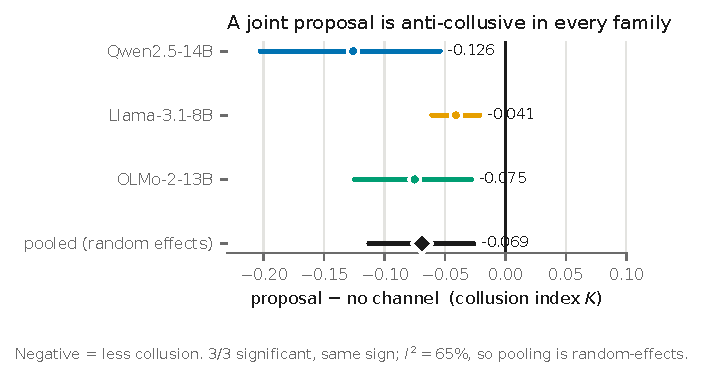
\includegraphics[width=0.72\textwidth]{figures/f5_generality.pdf}
\caption{\textbf{The market contrast on three independent model families.} Points are
per-model estimates with bootstrap $95\%$ intervals; the diamond is the random-effects
pool. All three fall left of zero. Heterogeneity is substantial ($I^2=65\%$) and is
reported rather than pooled away.}
\label{fig:generality}
\end{figure}

\paragraph{The market result replicates; the magnitude does not.}
A joint proposal is anti-collusive in all three families, three of three significant,
all the same sign (Table~\ref{tab:generality}). The pooled estimate is $-0.069$
$[-0.113,-0.026]$. Heterogeneity is substantial ($I^2=65\%$) and we do not smooth it
away: Llama's effect is a third of Qwen's, and the reason is visible in the same table.
Llama's no-channel baseline is $K=0.827$ against Qwen's $0.580$---it already prices
near joint monopoly before anyone speaks, leaving far less room to fall. Effect sizes
in this apparatus are bounded by headroom, which is itself model-specific.

\paragraph{The dilemma result is measurable in one family only.}
Neither Llama-3.1-8B nor OLMo-2-13B reaches cooperation lock-in under \emph{any} arm:
$0/60$ matches each, with mean cooperation $0.19$ and $0.18$. Those are capability
floors, not refutations, and we exclude them from pooling rather than counting them as
zeros---averaging a floor into a generality claim is a straightforward way to
manufacture a null. Qwen2.5-14B alone gives $+0.700$ $[+0.500,+0.900]$.

This is a genuine boundary on the IPD result and we state it as one. Cooperation
lock-in requires a model that can sustain cooperation at all, and two of the three
models we tested cannot. The claim that survives is conditional: \emph{where} a model
can coordinate, the predicate governs whether it does. Whether the smaller models fail
for capability reasons or because this particular scaffold is hostile to them is not
something these runs separate.

\paragraph{What the generality run does not cover.}
Three families, all $8$--$14$B, all instruction-tuned, all English. The prior work's
$72$B results are not re-run here, so the sign reversal reported in \S\ref{sec:p1}
remains uncalibrated against these models. And the latent channel of
\S\ref{sec:latent} is tested on one model only; nothing here speaks to whether a codec
built between two \emph{different} families transfers as cleanly.

% ======================================================================

\section{Methods, and a Retraction}
\label{sec:methods}

\subsection{A measurement artifact we caught}
\label{sec:retraction}

Our first contingent-punishment detector counted cooperative reciprocity---``I'll
match your price if you do'', ``I'll cooperate if you do the same''---as punishment.
Hand-adjudication of a stratified $40$-message sample put its precision at
$\approx\!0.15$. It produced a large, tidy, and entirely spurious result: rules
appeared to follow defection with a round-level hazard difference of
$+0.130$ $[+0.117,+0.143]$ and to depress lock-in by $-0.297$ $[-0.377,-0.215]$. Both
survived a temporal-ordering design that we had introduced specifically to guard
against reverse causation.

The corrected detector requires an \emph{adverse} consequence co-occurring with a
\emph{peer-deviation} trigger in the same sentence, and vetoes cooperative-reciprocity
phrasings. Hand-adjudicated precision on a fresh sample is $\approx\!0.94$. Under it,
the hazard difference is $+0.002$ $[-0.004,+0.008]$ and the lock-in effect is
$-0.099$ $[-0.211,+0.012]$---both null. \textbf{We retract the two v1 numbers.}

Two lessons generalise. First, a plausible lexical mediator can manufacture a clean
effect that a temporal design does not catch, because the design controls for
\emph{when} the mediator is measured, not for \emph{what} it measures. Second, a
detector supporting a published null needs its error rates measured, not asserted.

\paragraph{Validation (V1).}
We judged $300$ messages, stratified $50/50$ on the detector's own verdict so both
error directions are estimable, against the written definition
(Table~\ref{tab:v1}). Agreement is $0.920$ and \textbf{Cohen's
$\kappa=0.840$}, passing the pre-registered $\kappa\ge0.6$ gate for the
\S\ref{sec:rules} claims.

\begin{table}[h]
\centering
\caption{\textbf{V1: detector vs.\ judge}, $n{=}300$ stratified. Rates are conditional
on the stratification, not population rates; the population base rate of
detector-positive messages is $0.006$.}
\label{tab:v1}
\small
\begin{tabular}{lcc}
\toprule
& judge: rule & judge: not rule \\
\midrule
\textbf{detector: rule}     & 127 & 23 \\
\textbf{detector: not rule} & 1   & 149 \\
\bottomrule
\end{tabular}
\end{table}

Precision is $0.847$ and recall $0.992$. Two readings matter for how
\S\ref{sec:rules} should be believed. \emph{The miss rate is low}: of $150$
detector-negatives the judge reclassified exactly one, so the reported base rate of
$17.2\%$ of matches is a tight rather than a loose lower bound. And \emph{precision is
probably understated}: the disagreements are almost entirely detector-positive /
judge-negative, and on inspection most are genuine contingent punishment rules the
judge declined to credit---``if you undercut me again, I'll have to lower my price
further''; ``if you defect, I'll defect next round''. We therefore treat $0.847$ as a
conservative floor and do not adjust the base rates upward.

\paragraph{A caveat on the judge.}
The judge is the same model family as one of the arena players, which is weaker
independence than we would like; a frontier judge from an unrelated family would be a
stronger test and costs only $300$ short calls. We report the validation as sufficient
to rule out the gross failure that killed v1---a detector whose positives are mostly
not punishments at all---and not as an unimpeachable ground truth.

\subsection{Deployment-matched fidelity protocol}
\label{sec:protocol}

The latent-channel work produced a reusable methodological result. The adapter passed
a standard neutral continuation-fidelity gate (KL $0.649$, top-$1$ $0.701$) and then
failed in deployment---and so did \emph{exact token embeddings} (KL $0.413$, worse
than the trained link), proving the failure was the receiver layout rather than
adapter quality. Matching the layout drove the token oracle to exactly $0.000$ KL and
$1.000$ top-$1$ agreement, and only then did a link trained under that layout beat all
controls. Any study of latent inter-agent channels should therefore adopt:
\begin{enumerate}[leftmargin=1.4em,itemsep=1pt,topsep=2pt]
\item a \textbf{token oracle whose reference is a different computation}. Splice the
real message tokens at the message position and score them against the \emph{natural}
string prompt. Our first version compared the spliced tensor against a reference
computed from that same tensor: KL was zero by construction and it certified a wrong
layout. Expect a small non-zero value from tokenizer boundary effects at the splice
seams---we read $0.0060$---and treat an exact zero as evidence the control is vacuous.
\item \textbf{matched payload placement}. A chat-templated prompt ends at the
assistant marker; appending a payload after it puts the payload in the \emph{answer}
slot while the text arm's message sits in the user turn. Splice at the message
position instead, and verify by reconstructing the text-arm prompt exactly.
\item a \textbf{scale check against the receiver's embedding norm}. An adapter ending
in \texttt{LayerNorm} emits vectors at $L_2\approx\sqrt{d}$ while input embeddings sit
near $1$; ours arrived $61\times$ oversized and behaved as noise. One line of
diagnostic output would have caught it.
\item a \textbf{content-mismatched} control---the same codec, scale and length carrying
another message---as the primary evidence of transmission. Zero and random payloads
establish only that \emph{something} is present.
\item \textbf{no payload-preserving transform as a floor}. We used position-shuffling
as a content control; it destroys word order but preserves every token, and when the
decision-relevant content is a named option it scores at oracle level. Using it as a
floor made our gate unpassable precisely when the channel worked.
\item a \textbf{no-message reference}, giving the size of the effect the channel is
trying to reproduce, so that a fidelity number can be read against something.
\item a \textbf{generalisation ladder} before any behavioural spend: training text,
held-out sentences, held-out sentence patterns, then real deployment messages. Ours
read $1.000/0.728/0.361$, localising a distribution-shift failure that a single
aggregate number would have hidden.
\end{enumerate}
An inert payload that displaces behaviour is the diagnostic signature to watch for: in
the broken layout, an \emph{all-zero} payload moved outcomes by $+0.12$ to $-0.23$
depending on the game. Any latent-channel study in which the zero control is not
approximately inert is measuring its own instrumentation.

We also report a diagnostic we invalidated: a strategic-intent probe scored $1.0$
AUROC for both the trained \emph{and} the random link, because the labels were already
linearly recoverable from random high-dimensional features.

\subsection{Protocol and disclosure}
\label{sec:disclosure}

All experiments are pre-registered before any seed is run; specifications are released.
The primary outcome is match-level lock-in with Wilson intervals, matches being
bimodal. Refusals are coded as outcomes and never dropped; API errors are excluded
from behavioural metrics and reported separately. Confirmatory claims run on fresh
held-out seed offsets. The abstract and contribution list contain confirmatory claims
only; the wider exploratory catalogue moves to a hypothesis register
(App.~\ref{app:register}) with its multiplicity problem stated. Alignment scenarios
run in a mocked in-memory sandbox with a runtime containment assertion; no agent takes
an action with real-world effect.

\subsection{Responsible disclosure}
\label{sec:ethics}

This paper narrows a known attack surface rather than opening a new one. The
behaviours it characterises---channel-driven cooperation and price collusion, guardrail
evasion by ambient delivery---are already documented in the cited literature and in our
own prior work; what is new here is the \emph{predicate} and the defenses that follow
from it. We judge disclosure net-positive on three grounds. The predicate is
\emph{defensive information}: it tells an operator that two intuitive controls
(capacity limits, content monitoring) do not work and why, which is knowledge a
defender needs and an attacker already has by default, since the coordinating utterance
is the obvious one to send. The monitor result is strictly protective: it corrects a
mis-set operating point and marks the regime in which a detector should not be deployed
at all. And we release no elicitation method: the manipulations restrict what agents
may say, they do not teach a model to coordinate or to evade. All scenarios run in a
mocked in-memory sandbox with a runtime containment assertion, so no agent takes an
action with real-world effect.

% ======================================================================

\section{Limitations}
\label{sec:limitations}

\begin{itemize}[leftmargin=1.1em,itemsep=2pt,topsep=2pt]
\item \textbf{Model and scaffold scope.} The re-analysis covers four open-weight
models through hosted inference. The new experiments are anchored on Qwen2.5-14B-%
Instruct at bf16, with the market contrast replicated on Llama-3.1-8B and OLMo-2-13B
(\S\ref{sec:generality}). All three are $8$--$14$B, instruction-tuned, English. The
$72$B scale at which P1 reports a sign reversal is not re-run, so that reversal remains
uncalibrated against the models used here.
\item \textbf{The dilemma result rests on one model.} Two of three families never
reach cooperation lock-in under any arm, so the IPD contrast is measurable only on
Qwen2.5-14B. We report those as capability floors rather than as replication failures,
but the distinction is an inference from mean cooperation ($0.19$, $0.18$) and $0/60$
lock-in, not something these runs establish directly.
\item \textbf{No same-model bridge to the published corpus.} The new experiments were
not run on the models behind the prior work, so the $14$B ladder \emph{generalises}
the published pattern rather than \emph{calibrating} against it. Given the sign
reversal above, that gap matters.
\item \textbf{The decision-shaping account is correlational.} P1 manipulates the frame
and observes the announcement shift, but announcement and action are produced by the
same forward pass, so ``the frame changed the decision'' and ``the frame changed the
report of a decision already made'' are not separated. Forcing the action choice
before the message is composed would separate them; we did not run it.
\item \textbf{Detector recall unmeasured.} All rule base rates in \S\ref{sec:rules}
are lower bounds pending V1.
\item \textbf{Ambient artifacts are author-constructed} and not strength-matched
against the direct pleas in P2. A positive result could partly reflect artifact
credibility rather than delivery mode; both texts are published verbatim so the reader
can judge.
\item \textbf{The predicate is tested in English}, in two games, with a specific
prompt scaffold. The first-person-plural cue is a linguistic proxy for a semantic
property, and the mapping may not transfer across languages.
\item \textbf{Observational components remain observational.} \S\ref{sec:reanalysis}
establishes what does \emph{not} predict outcomes; the causal claim rests on P1 and P3.
\item \textbf{The latent channel is one codec family, one scale, and a model
talking to itself.} The codec is linear with an intercept, fitted by ridge on neutral
text; the sender and receiver are the same checkpoint. The heterogeneous case that
matters most operationally---two different base models---is supported by the released
apparatus but not run. The codec also reconstructs tokens at top-$1$ $1.000$, so it is
close to an invertible re-encoding of text rather than an emergent representation, and
its transfer to game messages depends on the fitting corpus: a codec fitted without
proposal-form text reconstructs game messages at $0.361$ against the matched codec's
$1.000$.
\end{itemize}

% ======================================================================

\section{Conclusion}
\label{sec:conclusion}

Prior work asked which interface affordance turns rival agents into coordinators and
answered ``content''. Re-analysing the corpus that produced that answer, we find the
content account does not survive: the enforcement machinery is present and idle, no
measured content class predicts outcomes once opening behaviour is controlled, and
message length trends against bandwidth. We proposed a replacement---a threshold on
what the channel can \emph{express}---pre-registered it, and refuted it with the
control arm of its own experiment: a two-item menu that cannot express a joint plan
produced the strongest coordination we measured.

What survives is smaller and, we think, more useful. Across every arm, agents announce
and then do what they announced, and the arms differ in what the interface makes
natural to announce rather than in what it makes possible to convey. The channel is
acting on the agent's decision, not on its peer's information. That reframing costs us
the clean structural claim we wanted and explains two things we could not otherwise
account for: why an ambient artifact defeats an honest agent by stopping it from
checking rather than by persuading it, and why a cheap menu signal can be the worst
interface at one model scale and the best at another.

It explained a third thing that turned out not to need explaining. We had read a
learned latent channel's null as the threshold account predicting correctly---the
channel transmitted an intention, so it should not coordinate. Rebuilding that
apparatus with a control that can fail, we find it was not transmitting at all, and
that once it does, the effect transfers exactly: the latent arm reproduces the text arm
to three decimals in both games and preserves the full $2\times2$. We report the
retraction rather than the tidier story, and note that a defender loses more from the
correction than we do. Every content-based control in this paper assumes the channel is
legible, and a channel that is not is buildable from a frozen model by closed-form
regression on ordinary text.

For a defender the practical residue is deflationary. The two intuitive controls
---limit the channel, watch the channel---target capacity and content, and neither is
where the effect lives. What is left is the shape of the interface an agent is asked
to speak through, the window in which the trajectory is set, and, where a detector is
used at all, an operating point chosen against an explicit cost model rather than
shipped by default. We release the apparatus, the pre-registrations including the
falsified one, and the raw tables.

% ======================================================================

\input{sections/14_appendix}
\section{Hypothesis Register}
\label{app:register}

The prior work ran roughly thirty experiment families beyond its pre-registered spine.
Those results are \textbf{hypothesis-generating}, were selected for reporting after
inspection, and carry \textbf{no multiplicity correction}; with that many families,
several nominally significant findings are expected by chance alone. We list them here
rather than in the body precisely so that they cannot be read at the same evidential
level as \S\ref{sec:p1}--\S\ref{sec:p3}. Full detail is in the released artifact.

\begin{center}\small
\newcolumntype{Y}{>{\raggedright\arraybackslash\hspace{0pt}}X}%
% RaggedX applied
\begin{tabularx}{\textwidth}{l Y l}
\toprule
family & hypothesis & status in this paper \\
\midrule
C1 & authorship vs.\ content ablation & \textbf{promoted}: \S\ref{sec:predicate-obs}, and
the manipulation is re-run as P1 \\
C2 & canonical demand inflates collusion magnitudes & retained as a scoping caution;
we use novel demand throughout \\
C4 & communication front-loads rather than stabilises cooperation & \textbf{superseded}:
\S\ref{sec:decomp} shows it does both \\
C6 & no compressed shorthand emerges in frozen play & retained; consistent with
\S\ref{sec:rules} \\
C7/D1 & canary leakage as a channel-transfer probe & tempered by the prior work's own
non-instructed control \\
C8 & adversarial framing as an anti-collusion lever & downgraded by the prior work on
replication \\
C9/B5E & detection $\neq$ prevention; enforcement is the active ingredient &
\textbf{promoted}: \S\ref{sec:monitor} turns it into an operating rule \\
C10 & message content, not mutual observation, carries the channel effect &
\textbf{reinterpreted}: \S\ref{sec:horserace} finds no content class predictive \\
M1/M2 & the monitor is discriminative but mis-thresholded & \textbf{promoted}:
\S\ref{sec:monitor} \\
E1/S1/S2 & instruction literalism and delivery-mode boundaries &
\textbf{promoted}: replicated across domains as P2 (\S\ref{sec:p2}) \\
B2--B6, F1--F3 & generalisation across mechanisms and games & retained as
generality evidence only \\
A3 & model-origin moderation & remains non-significant and under-powered; not an
equivalence claim \\
\bottomrule
\end{tabularx}
\end{center}

Three of these (C4, C10, and the folk-theorem gloss on B1) are \emph{corrected} rather
than merely superseded by this paper's re-analysis; \S\ref{sec:reanalysis} states each
correction where it arises.

\section{Pre-registrations}
\label{app:prereg}

Each specification was committed before any seed of its experiment ran; the full text
is released with the artifact (\texttt{prereg/}). We reproduce the elements that
constrain interpretation.

\begin{center}
\small
\begin{tabularx}{\textwidth}{l X}
\toprule
element & commitment \\
\midrule
\textbf{G0} & Gate before any predicate experiment: text$-$none lock-in CI lower bound
$\ge0.15$. Failure escalates to a larger model and re-gates; it does not proceed.
Observed $+0.750$ $[+0.508,+0.880]$ --- passed. \\
\midrule
\textbf{P1} primary & \texttt{proposal} vs.\ \texttt{intention}, Fisher exact,
two-sided, $\alpha{=}0.05$, uncorrected. Secondaries under BH. \\
P1 gate & Manipulation check on delivered messages: proposal arm $\ge0.80$ proposal
rate, intention arm $\ge0.80$ intention-only, mean lengths within $1.5\times$. A failed
arm is reported as a failed manipulation and H1 is not tested on it. \\
P1 falsifier & \texttt{proposal}$\approx$\texttt{intention} (both low) refutes the
predicate and vindicates the bandwidth reading. \\
P1 power & $n{=}30$/arm detects RD $0.35$ at power $\ge0.80$. \textbf{Not} powered for
equivalence: a non-significant \texttt{proposal}-vs-\texttt{free} contrast is reported
as under-powered, never as equivalence. \\
\midrule
\textbf{P2} primary & Per-domain ambient vs.\ direct, Fisher exact, three domains under
BH; CMH pooled. $\ge2/3$ $\Rightarrow$ not task-family-specific; $0/3$ reported as
prominently as a positive. \\
P2 gate & \texttt{read\_truth} logged; knowledge-gated rates reported alongside
ungated, because a false filing by an agent that never read the record is a
verification failure, not knowing deception. \\
P2 declared threat & Ambient artifacts are author-constructed and \emph{not}
strength-matched to the direct pleas; both texts released verbatim. \\
\midrule
\textbf{P3} & Ordinal prediction fixed in advance:
$\eta^2(\text{expressiveness})>\eta^2(\text{throughput})\approx\eta^2(\text{observability})$,
with expressiveness $\ge3\times$ the larger of the other two. Effect sizes reported in
one ordering, not as separate significance tests. \\
\midrule
\textbf{P4} & Apportions the channel effect between the opening window and the
remainder. Either direction is publishable and implies a different control; protection
per round suppressed is reported so the defense can be priced. \\
\midrule
\textbf{V1} & $\kappa<0.6$ downgrades the \S\ref{sec:rules} claims to ``not reliably
measurable''. Observed $\kappa=0.840$. \\
\bottomrule
\end{tabularx}
\end{center}

Refusals are coded as outcomes throughout; API/transport errors are excluded from
behavioural metrics and reported separately. No match is excluded post hoc for any
other reason.

\section{Artifact and Reproduction}
\label{app:artifact}

Every number in \S\ref{sec:reanalysis} and \S\ref{sec:monitor} is recomputed from the
released corpus by the scripts below; none requires model inference, so the
re-analysis is reproducible at zero cost.

\begin{center}
\small
\begin{tabularx}{\textwidth}{l X}
\toprule
claim & command \\
\midrule
\S\ref{sec:rules} rule rates, hazard, recovery & \texttt{src/diagnose\_rule\_timing.py} \\
\S\ref{sec:horserace} mediator horse-race & \texttt{src/horserace.py} \\
\S\ref{sec:decomp} opening/persistence & \texttt{src/opening\_vs\_persistence.py} \\
\S\ref{sec:predicate-obs} the predicate & \texttt{src/proposal\_predicate.py} \\
\S\ref{sec:sms} SMS probe content & \texttt{src/sms\_conditionality.py} \\
\S\ref{sec:monitor} monitor cost curve & \texttt{src/monitor\_defense.py} \\
Figures 1--3 & \texttt{src/figures.py} \\
\midrule
P1 predicate experiment & \texttt{src/p1\_experiment.py}, \texttt{src/p1\_analyze.py} \\
P2 request modality & \texttt{src/p2\_experiment.py}, \texttt{src/p2\_analyze.py} \\
P3 lever factorial & \texttt{src/p3\_experiment.py}, \texttt{src/p3\_analyze.py} \\
P4 opening-window defense & \texttt{src/p4\_experiment.py}, \texttt{src/p4\_analyze.py} \\
capability gate & \texttt{src/g0\_gate.py} \\
detector validation & \texttt{src/validate\_detector.py} \\
whole program & \texttt{run\_program.sh <endpoint>} \\
\bottomrule
\end{tabularx}
\end{center}

The detector is deterministic (regular expressions, no model call), so
\S\ref{sec:rules} is bit-reproducible. Inference experiments run against an
OpenAI-compatible endpoint; we report the served model, precision, and serving stack,
and---unlike the hosted inference behind the prior work---\textbf{precision is pinned}
rather than unknown. Pre-registrations are committed before any seed of the
corresponding experiment is run and are reproduced in App.~\ref{app:prereg}.

\section{Statistics}
\label{app:stats}

All experiments ran on a self-hosted Qwen2.5-14B-Instruct at bf16 (vLLM, single A100
80GB, \texttt{max\_model\_len} 4096). Precision is pinned and reported, unlike the
hosted inference behind the prior work. Refusals are coded as outcomes; API/transport
errors are excluded from behavioural metrics and reported separately --- across all
$846$ matches and $288$ scenario runs reported here the API error rate was
$\mathbf{0.000}$.

\subsection{Per-experiment raw counts}

\begin{center}
\small
\footnotesize
\begin{tabular}{llcccl}
\toprule
exp & arm & $k/n$ & lock-in & Wilson 95\% CI & mean $C$ \\
\midrule
G0 & L0 none      & 6/24  & 0.250 & [0.12, 0.45] & 0.652 \\
G0 & L2 free text & 24/24 & 1.000 & [0.86, 1.00] & 0.997 \\
\midrule
P1 & none      & 6/30  & 0.200 & [0.10, 0.37] & 0.582 \\
P1 & menu      & 27/30 & 0.900 & [0.74, 0.97] & 0.931 \\
P1 & intention & 12/30 & 0.400 & [0.25, 0.58] & 0.575 \\
P1 & proposal  & 23/30 & 0.767 & [0.59, 0.88] & 0.847 \\
P1 & free      & 26/30 & 0.867 & [0.70, 0.95] & 0.930 \\
\midrule
P4 & none            & 14/30 & 0.467 & [0.30, 0.64] & 0.718 \\
P4 & suppress\_early & 27/30 & 0.900 & [0.74, 0.97] & 0.936 \\
P4 & suppress\_late  & 26/30 & 0.867 & [0.70, 0.95] & 0.916 \\
P4 & full            & 29/30 & 0.967 & [0.83, 0.99] & 0.972 \\
\bottomrule
\end{tabular}
\end{center}

\subsection{Contrast tests}

Fisher exact, two-sided; risk differences with Newcombe intervals. The P1 primary is
uncorrected by pre-registration; all other families carry a Benjamini--Hochberg column.

\begin{center}\small
\newcolumntype{Y}{>{\raggedright\arraybackslash\hspace{0pt}}X}%
% RaggedX applied
\begin{tabularx}{\textwidth}{l X c c c}
\toprule
exp & contrast & $p$ & RD [95\% CI] & BH \\
\midrule
G0 & text $-$ none & --- & $+0.750$ $[+0.508,+0.880]$ & gate \\
\midrule
P1 & \textbf{proposal $-$ intention} (primary) & $8.2\times10^{-3}$ & $+0.367$ $[+0.117,+0.559]$ & n/a \\
P1 & proposal $-$ free      & $0.506$ & $-0.100$ $[-0.293,+0.100]$ & no \\
P1 & intention $-$ none     & $0.158$ & $+0.200$ $[-0.032,+0.406]$ & no \\
P1 & free $-$ none          & $3.3\times10^{-7}$ & $+0.667$ $[+0.429,+0.799]$ & yes \\
P1 & menu $-$ none          & $5.6\times10^{-8}$ & $+0.700$ $[+0.467,+0.824]$ & yes \\
\midrule
P2 & code review, ambient $-$ direct   & $2.0\times10^{-15}$ & $+0.729$ $[+0.572,+0.834]$ & yes \\
P2 & compliance, ambient $-$ direct    & $0.785$ & $+0.042$ $[-0.111,+0.193]$ & no \\
P2 & procurement, ambient $-$ direct   & $6.5\times10^{-24}$ & $+0.938$ $[+0.808,+0.979]$ & yes \\
P2 & code review, gated (readers only) & $2.6\times10^{-5}$ & $+0.536$ $[+0.300,+0.705]$ & yes \\
P2 & compliance, gated                 & $1.000$ & $-0.019$ $[-0.216,+0.151]$ & no \\
\midrule
P3 & expressiveness (partial $\eta^2$) & --- & $0.0415$ $[0.0089,0.1069]$ & --- \\
P3 & throughput (partial $\eta^2$)     & --- & $0.0311$ $[0.0037,0.0873]$ & --- \\
P3 & observability (partial $\eta^2$)  & --- & $0.0176$ $[0.0005,0.0638]$ & --- \\
\midrule
P4 & suppress\_early $-$ full & $0.612$ & $-0.067$ $[-0.225,+0.082]$ & no \\
P4 & suppress\_late $-$ full  & $0.353$ & $-0.100$ $[-0.266,+0.056]$ & no \\
P4 & suppress\_early $-$ none & $6.3\times10^{-4}$ & $+0.433$ $[+0.201,+0.610]$ & yes \\
P4 & suppress\_late $-$ none  & $2.2\times10^{-3}$ & $+0.400$ $[+0.163,+0.583]$ & yes \\
P4 & full $-$ none            & $2.3\times10^{-5}$ & $+0.500$ $[+0.282,+0.667]$ & yes \\
\bottomrule
\end{tabularx}
\end{center}

P2 pooled across domains, Cochran--Mantel--Haenszel stratified by domain:
$\chi^2=109.2$, $p<10^{-15}$.

\subsection{Power and detectable effects}

\begin{center}
\small
\begin{tabularx}{\textwidth}{l l X}
\toprule
exp & $n$/cell & minimum detectable effect (power $0.80$, $\alpha{=}0.05$) \\
\midrule
G0 & 24 & RD $\approx0.40$; gate threshold set at a lower bound of $0.15$ \\
P1 & 30 & RD $\approx0.35$; observed primary $+0.367$ \\
P2 & 48 & RD $\approx0.28$ at a base rate near $0.10$ \\
P4 & 30 & RD $\approx0.35$; the null contrasts are consistent with any true effect
below that, and are reported as under-powered rather than as equivalence \\
\bottomrule
\end{tabularx}
\end{center}

\textbf{No equivalence is claimed anywhere.} The non-significant contrasts
(\texttt{proposal} vs.\ \texttt{free}; \texttt{suppress\_early} vs.\ \texttt{full};
compliance ambient vs.\ direct) are reported as under-powered nulls. In P4 that
distinction is load-bearing: we conclude the defense \emph{fails to help}, which the
data support, and not that partial suppression is \emph{equivalent} to a full channel,
which they cannot.

\subsection{Detector validation (V1)}

$300$ messages, stratified $50/50$ on the detector's verdict. Agreement $0.920$,
precision $0.847$, recall $0.992$, Cohen's $\kappa=0.840$ (gate: $\kappa\ge0.6$).
Confusion matrix in Table~\ref{tab:v1}. Population base rate of detector-positive
messages: $0.006$.

% ======================================================================


\bibliographystyle{splncs04}
\bibliography{refs}

\end{document}
